\documentclass[a4paper]{article}

\usepackage{amsmath}
\usepackage{amssymb,amsfonts}
\usepackage[catalan]{babel} % Language 
\usepackage{fontspec}
\usepackage[margin=2cm]{geometry}
\usepackage{graphicx}
\usepackage[makeroom]{cancel}
\usepackage{listings}
\usepackage[dvipsnames]{xcolor}
\usepackage{float}
\usepackage{enumitem}
\usepackage[hidelinks]{hyperref}

\setlength{\parindent}{0pt}
\setlength{\parskip}{0.2cm}

\title{\textsc{APA Problemes} \\ Problema 8 Mínims quadrats}
\author{Joan Marcè i Igual}
\date{}

\begin{document}
\maketitle

\begin{enumerate}
    \item \textbf{Calculeu la matriu de covariància mostral de les dades $\Sigma$.}
\end{enumerate}

$\Sigma = \frac{1}{N} \sum_{n=1}^N \left((\vec{X}_n - \vec{\mu})(\vec{X}_n - \vec{\mu})^T\right)$

\begin{flalign*}
\text{En particular } & CoVar(X_i, X_j) = \sigma_{ij}^2 &\\
& CoVar(X_i, X_i) = \sigma_{ii}^2 = Var(X_i) =\sigma_i^2 &
\end{flalign*}

$$
\Sigma =
\begin{pmatrix}
7,143 & 4.857 \\
4.857 & 4.000
\end{pmatrix}
$$


\begin{enumerate}[resume]
    \item \textbf{Calculeu els dos valors propis de $\Sigma$}
\end{enumerate}

Usant la comanda \verb|eigen| de \textbf{R} es poden obtenir els valors propis d'una matriu. Així doncs els valors propis de $\Sigma$ són $\lambda_1 = 10,676$ i $\lambda_2 = 0,466$.

\begin{enumerate}[resume]
    \item \textbf{Calculeu els dos vectors propis corresponents $\vec{a}_1$ i $\vec{a}_2$.}
\end{enumerate}

Els valors propis també es poden obtenir a partir de la comanda \verb|eigen| usada a l'apartat anterior

$$
\vec{a}_1 =
\begin{pmatrix}
-0,809 \\
-0,588
\end{pmatrix} \quad
\vec{a}_2 =
\begin{pmatrix}
0,588 \\
-0,809 
\end{pmatrix}
$$

Es pot comprovar que els dos vectors són perpendiculars fent el producte escalar:
$$
\vec{a}_1 · \vec{a}_2 = -0.476 + 0.476 = 0
$$

\begin{enumerate}[resume]
    \item \textbf{Dibuixeu les dades i les dues components principals}
\end{enumerate}

\begin{figure}[H]
    \centering
    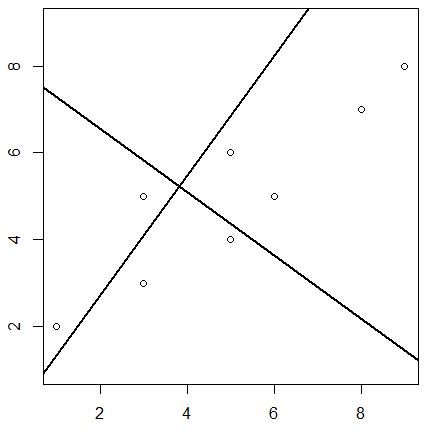
\includegraphics[width=0.5\textwidth]{Rplot}
\end{figure}

\begin{enumerate}[resume]
    \item \textbf{Quin és el percentatge de variància explicada per la primera component principal?}
\end{enumerate}

$$ 
\%\text{de variància retinguda } = \frac{\sum_{i=1}^k \lambda_i}{\sum_{i=1}^d \lambda_i}·100 =
\frac{10,676}{11,143} = 95,814 \%
$$

\end{document}